\section{Introduction}
Modern software systems involve intricate changes that extend far beyond source code modifications. A significant portion of system behavior is governed by configuration files, encompassing deployment scripts, service settings, infrastructure definitions, and more. Ensuring the correctness of these configurations is critical, yet challenging. Software vendors often provide extensive manuals to guide administrators, but the length and complexity of these documents can be prohibitive, frequently leading practitioners to guess when configuring systems \cite{Xiang.2020}. This challenge is compounded by the rapid pace of technological evolution, which necessitates constant updates to configuration schemes.

The consequences of misconfiguration can be severe, significantly contributing to production bugs and system failures, as highlighted by large-scale studies \cite{Tang.2015}. Traditionally, validating configurations has relied on methods such as static analysis, integration testing, and manual review \cite{Lian.2024}. While valuable, these approaches often struggle to keep pace with the complexity and dynamism of modern software environments. Furthermore, the scale at which validation is required can be immense; Facebook, for example, reported executing trillions of configuration checks daily \cite{Tang.2015}. This necessitates solutions that are not only accurate but also highly performant and resource-efficient, implying that evaluation solely based on metrics like precision or recall is insufficient. Consequently, there is a pressing need for more automated, reliable, and scalable validation techniques.

Retrieval-Augmented Generation (RAG) systems offer a promising approach to address this gap. By combining the knowledge retrieval capabilities of search systems with the reasoning power of Large Language Models (LLMs), RAG can potentially interpret complex technical documentation (like configuration manuals) and apply this understanding to validate specific configurations against best practices or requirements.

This chapter aims to demonstrate the practical application of the RAGBench evaluation framework, detailed in Chapter 4, to the specific problem of configuration validation. We will leverage this framework to systematically evaluate the performance of various RAG configurations against established baselines using an extended version of the CTest dataset \cite{Lian.2024}, which includes synthetically generated examples. While acknowledging that configuration validation is a multifaceted problem involving aspects like inter-configuration dependencies, this experiment focuses specifically on validating individual configuration settings based on documented guidelines.

The remainder of this chapter is structured as follows: Section \ref{sec:related_works_exp} discusses related work in applying RAG to software engineering tasks, particularly configuration validation. Section \ref{sec:exp_design_exec} details the experiment design, including the dataset, baselines, RAG configurations, evaluation metrics, and tools used, adhering to the methodology outlined in Chapter 4. Section \ref{sec:exp_results} presents and analyzes the results obtained on the validation and test sets, including end-to-end performance, component analysis, and failure analysis. Section \ref{sec:exp_discussion} discusses the overall findings and their implications. Finally, Section \ref{sec:exp_conclusion} summarizes the key outcomes of the experiment.
% Note: Added \label tags for section references - adjust as needed if you rename sections.

\section{Related Works} \label{sec:related_works_exp}
Several approaches have been developed for validating software configurations.

Specification-based frameworks, such as ConfValley \cite{Huang.2015}, function by having engineers define validation rules explicitly, often in a declarative manner. Configuration Testing validates configuration values by executing the software components that use these values and observing the resulting program behavior \cite{XudongSun.2020}. This method is used to detect the dynamic effects of configuration settings and identify errors.

Lian et al. \cite{Lian.2024} introduced Ciri, a method that uses Large Language Models for configuration validation. Ciri employs prompt engineering and few-shot learning, providing the LLM with examples of both valid and invalid configurations alongside relevant documentation snippets to identify misconfigurations. This work applies Retrieval-Augmented Generation to the configuration validation task presented by Lian et al. \cite{Lian.2024}. We utilize the RAGBench evaluation framework chapter \ref{chap:design} to systematically assess and reconfigure different RAG systems for this specific task, aiming to optimize their performance through iterative refinement.

\section{Experiment Design and Execution} \label{sec:exp_design_exec}
The following sections detail the design and execution of our configuration validation experiment, adhering strictly to the methodology established by the RAGBench framework presented in Chapter \ref{chap:design}. The core principle involves splitting the evaluation dataset into validation and test sets, performing all system configuration, evaluation, and iterative refinement exclusively on the validation set, and finally assessing generalization on the held-out test set. Specifically, we employ a 70/30 validation-test split for the extended CTest dataset to ensure a sufficiently large test set for estimating generalization error (Section \ref{sec:valtestsplit}).

Our experimental workflow begins by establishing performance baselines using a standalone LLM and a naive RAG system (Section \ref{sec:framework-baselines}). We then evaluate an initial RAG configuration. Subsequent steps involve analyzing performance bottlenecks and failures using the framework's end-to-end and component-level metrics, alongside detailed trace analysis facilitated by MLflow and Langfuse (Section \ref{sec:evaluation-techniques}). Insights from this analysis guide iterative reconfiguration cycles aimed at improving performance on the validation set.

A key difference in our evaluation approach compared to the original Ciri experiment \cite{Lian.2024} lies in handling output formatting. While Ciri reran queries until a correctly formatted answer was obtained, our framework employs a strict format check; if the generator's output does not conform to the expected format (e.g., providing a clear "valid" or "invalid" classification alongside reasoning, as per Section \ref{sec:generator-evaluation}), the response is marked as incorrect for the purpose of end-to-end metric calculation. This reflects a scenario where automated post-processing requires predictable output.

% Differences Ciri to Me:
% They run it as long as it needs to get the correctly formatted answer
% I check with format_checker if the format is correct, otherwise its false

% Start with baselines and an RAG with trivial prompt
% Check for bottlenecks via MLFlow and Langfuse
% <Reiterate here a bit out of the typical experiment workflow showed in 40_DEsign_of_Valid_RAG_Evaluation.tex>

% We will use a 70/30 Validation Test Split for having enough on the test set to estimate correctly


\subsection{Experimental Setup} \label{sec:exp_setup}
The experiments were conducted using the computational resources specified below. The primary environment for running the evaluation framework, including data processing, baseline evaluations, and RAG pipeline executions involving API-based LLMs or CPU-based components, was a dedicated server hosted by Hetzner. We haven chosen closed as well as open source models and used \\OpenRouter.ai\cite{openrouter-inc-2023} for all API requests. We chose not to self-host a model by ourself, because this would skew system metrics such as latency.

We chose the CCX23 dedicated CPU server\cite{hetzner-online-gmbh-2025} for all our tests
\begin{itemize}
    \item VCPU: 4
    \item RAM: 16 GB
    \item SSD: 160 GB
\end{itemize}

\paragraph{Dataset} 
We used the CTest dataset, prepared by the team behind Ciri\cite{Lian.2024}\cite{xlab-uiuc-2025}. The data consists of real world missconfiguration scenarios, augmented with synthetic data. We had 907 test cases in total. In the following table is the distribution per system.

\begin{table}[h]
    \centering
    \begin{tabular}{|l|c|c|}
        \hline
        \textbf{Technology} & \textbf{Number of Files} & \textbf{Version} \\
        \hline
        alluxio & 111 & 2.5.0 \\
        django & 36 & 4.0.0 \\
        etcd & 64 & 3.5.0 \\
        hbase & 107 & 2.2.7 \\
        hcommon & 138 & 3.3.0 \\
        hdfs & 149 & 3.3.0 \\
        postgresql & 62 & 13.0 \\
        redis & 88 & 7.0.0 \\
        yarn & 80 & 3.3.0 \\
        zookeeper & 72 & 3.7.0 \\
        \hline
    \end{tabular}
    \caption{Number of configuration files and versions per system.}
    \label{tab:technology_values}
\end{table}

We then defined the validation-test split paramter. We chose a test size of 20 \%, resulting in 725 validation data points and 182 test data points.  

The ingestion of data into our vector database required scraping official documentation for each specific version. However, we could not find documentation or a manual for this specific Redis version as well as for hbase, hcommon and hdfs. Table \ref{tab:technology_documentation} shows the documentation sources we scraped.

\begin{table}[h]
    \centering
    \begin{tabular}{|l|l|}
        \hline
        \textbf{Technology (Version)} & \textbf{Documentation Page} \\
        \hline
        alluxio (2.5.0) & \texttt{https://docs.alluxio.io/os/javadoc/2.5/} \\
        django (4.0.0) & \texttt{https://docs.djangoproject.com/en/4.0/} \\
        etcd (3.5.0) & \texttt{https://etcd.io/docs/v3.5/} \\
        \textbf{hadoop-} & \texttt{https://hadoop.apache.org/docs/stable/}\\
        & \hspace{0.25cm} \texttt{hadoop-project-dist/} \\
        \hspace{0.15cm} hbase (2.2.7) & \hspace{0.5cm} \texttt{hadoop-common/} \\
        \hspace{0.15cm} hcommon (3.3.0) & \hspace{0.5cm} \texttt{hadoop-common/} \\
        \hspace{0.15cm} hdfs (3.3.0) & \hspace{0.5cm} \texttt{hadoop-hdfs/} \\
        postgresql (13.0) & \texttt{https://www.postgresql.org/docs/13/} \\
        redis (7.0.0) & \texttt{https://redis.io/docs/latest/commands/} \\
        yarn (3.3.0) & \texttt{https://hadoop.apache.org/docs/r3.3.0/} \\
        zookeeper (3.7.0) & \texttt{https://zookeeper.apache.org/doc/r3.7.0} \\
        & \hspace{0.25cm} \texttt{/apidocs/zookeeper-server/} \\
        \hline
    \end{tabular}
    \caption{Technology and Documentation Links}
    \label{tab:technology_documentation}
\end{table}

The ingestion of the data was ad-hoc before each experiment to have comparable results for ingestion times. 

\subsection{Reconfiguration Phases} \label{sec:exp_results} 

\paragraph{Initial Configuration and Baselines} \label{sec:exp_initial_config}
We used several baselines as comparison. At first we ran our experiment with the baselines defined in section \ref{chap:design} - as standalone LLM and a predefined minimal RAG system with BM25 sparse retrieval. For both baselines we used OpenAI's GPT-4o-mini\cite{OpenAI_2022}. The standalone system has only a generator and an answer builder for extracting "valid" or "invalid" from the generated output. The second baseline adds an retriever right before the generator and lists the top-10 documents before without any pre- or postprocessing. This basic architectures ensure that we figure out if complex adjustments improve the validator quality at all.

We also rebuilt the Ciri system within our Haystack RAG architecture and used it as baseline. As we only used our framework for running evaluations there are some minor differences in methodology due to implementation limitations. We did not look at the results per system, which means that we do not have knowledge if our system works better for django or alluxio systems. However we could run for each system a separat experiment, but we chose against for better comparability of the final result and cost reduction of the experiment. We also did only evaluate file-level validation. Ciri used few-shot examples with a number of valid and invalid configurations. We did not vary the number of valid or invalid shots, but we have chosen the best performing configuration with one valid and three invalid shots. Lastly Ciri used several language models for its experiments. We could just use \textit{gpt-3.5-turbo-0125}\cite{OpenAI_2022}. Other models were either unavaillable, because the used version is outdated and continuously trained or too expensive for the experiment to run with our budget. However we achieved a F1-Score of \textit{0.68} which close to the Ciri reported F1-Score of \textit{0.72}. All pipeline figures can be found in the appendix.

\subparagraph{Initial RAG Configuration} 
At first we tried different standalone LLMs for measuring the current state of LLM without complex system architecture. For our evaluation, we chose Qwen's \textit{QwQ-32B} \cite{qwq32b} and \textit{Qwen-2.5-coder-32b-instruct} \cite{hui2024qwen2}\cite{qwen2}\cite{qwen2.5}, OpenAI's versionized \textit{o1-mini}, \textit{gpt-4o-mini} version as well as an up-to-date version of \textit{gpt-4o-mini} for comparison. We also tested OpenAI's web-search version of \textit{gpt-4o-mini}, which appears to be an out-of-the-box RAG-system \cite{OpenAI_2022}. Lastly we added deepseeks most recent model \textit{V3} \cite{deepseekai2024deepseekv3technicalreport} to the list. 

Results can be seen in figure \ref{fig:LLMStandalone-Results}. The most recent \textit{GPT-4o-mini} model does perform best for F1-Score. The evaluated models to differ stronger on False-Positives-Rate and False-Negative-Rate than on F1-Scores. \textit{GPT-4o-mini} does have the lowest False-Negative-Rate and the highest False-Positive-Rate. Positives are valid configurations, so \textit{GPT-4o-mini} does classify invalid configurations more often as valid ones and does more rarely classify valid configurations as invalid. The older version of \textit{GPT-4o-mini} from 2024 and the web-search model have a slightly worse F1-Score, but more balanced FNR and FPR metrics. Even without few-shot learning as done by the Ciri team, the most recent version of \textit{gpt-4o-mini} did score an slightly higher average F1-Score ($0.6808$) than the configuration from the Ciri team with \textit{gpt-3.5-turbo-0125} ($0.6801$). In contrast to other models we did run the most recent version of gpt-4o-mini more frequently as baseline in later experiment runs. It now shows that the variance of the F1-Scores is with $1.41 \cdot 10^{-5}$ relatively small. 


\begin{figure}[h]
    \centering
    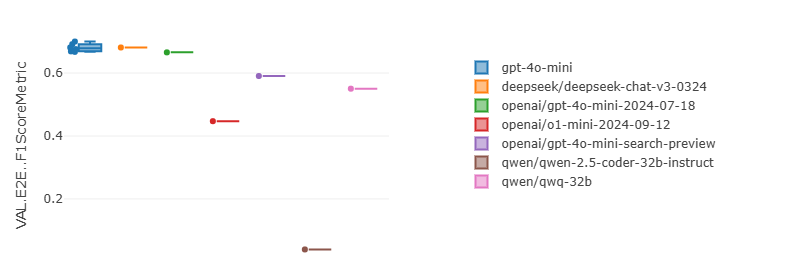
\includegraphics[width=0.95\textwidth]{images/LLMStandalone-by-model.png}\\[6pt]
    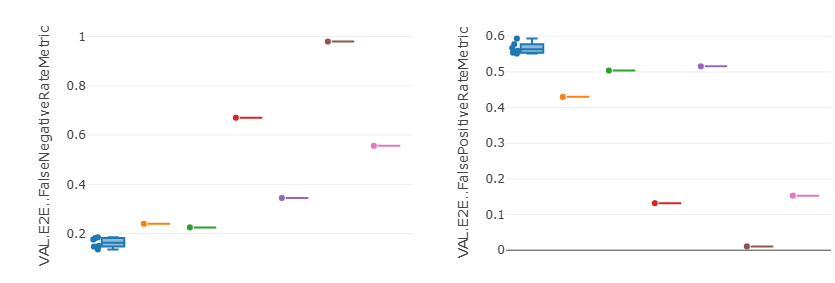
\includegraphics[width=\textwidth]{images/LLMStandalone-by-model-FNRFPR.png}
    \caption{Upper: F1-Score for standalone Large Language Models for configuration validation. }
    \label{fig:LLMStandalone-Results}
  \end{figure}

Next, we defined configurations for common retrieval techniques. A basic BM25 retriever is predefined as baseline. We also added one dense retriever with OpenAI's \textit{text-embedding-3-small}\cite{OpenAI_2022} and an hybrid version, which merges the results of the mentioned retriever with 3 different weight distributions with respect to the retrieved document list \textit{(1 ,2), (1, 1), (2, 1)}. We have evaluated the performance of these configurations with the both \textit{gpt-4o-mini-2024-08-06} and the most recent \textit{gpt-4o-mini} model. The results can be seen in figure \ref{fig:conf-phase-0-retrievers}. The results show that the selected model has more impact on the overall performance than the retrieval technique in this experiment. The retrieval metrics can be seen in table \ref{tab:retrieval_metrics}. Overall the sparse retriever performs better than the dense retriever. Both retrieval techniques perform poorly on retrieval quality. The weight distribution of the hybrid retriever had just a small impact on the performance, ranging F1-Score from \textit{0.567} to \textit{0.582}.

\begin{table}[h]
    \centering
    \begin{tabular}{|l|c|c|}
        \hline
        \textbf{Metric} & \textbf{BM25} & \textbf{Dense} \\
        \hline
        ContextRelevance & 0.3962 & 0.1761 \\
        MAP@K & 0.0964 & 0.0297 \\
        \hline
    \end{tabular}
    \caption{Retrieval metrics comparison between BM25 and Dense retrieval}
    \label{tab:retrieval_metrics}
\end{table}

\begin{figure}[!ht]
    \centering
    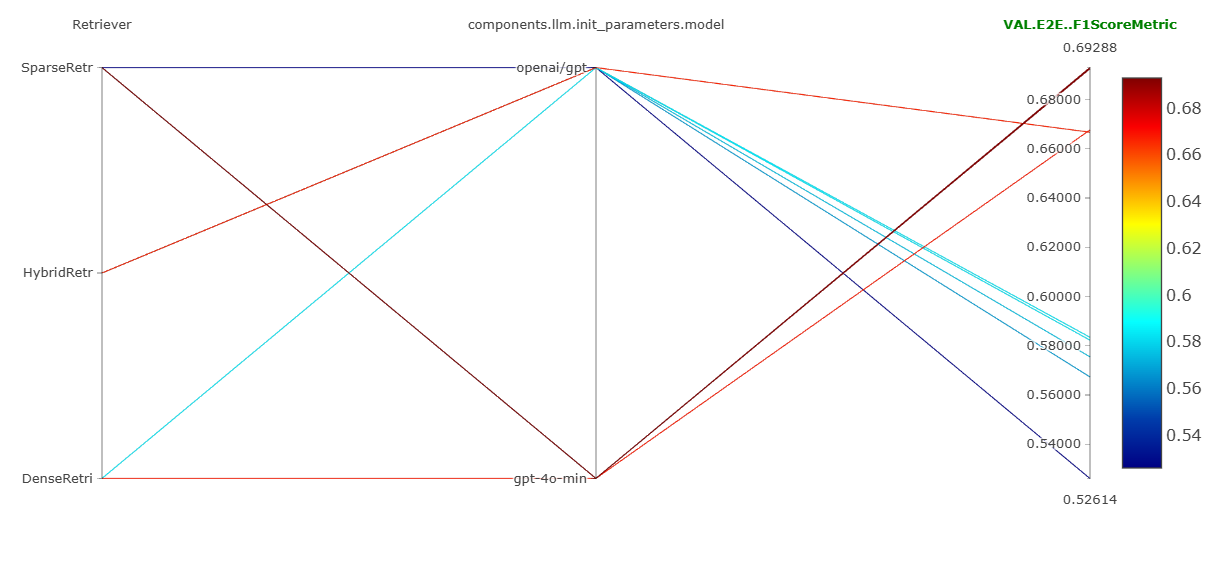
\includegraphics[width=\textwidth]{images/RetrievalTypes-vs-LLM-f1.png}\\[6pt]
    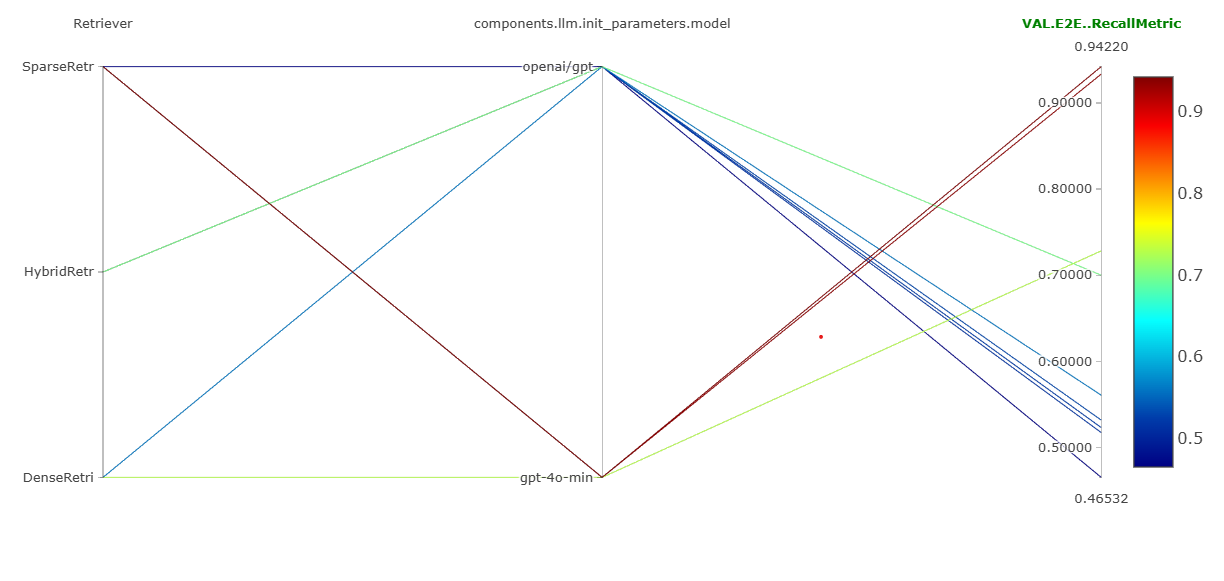
\includegraphics[width=\textwidth]{images/RetrievalTypes-vs-LLM-Recall.png}
    \caption{Experiments with different retrieval techniques and models. In both figures the upper model is the versionized \textit{gpt-4o-mini} and the lower model is the most recent \textit{gpt-4o-mini}.}
    \label{fig:conf-phase-0-retrievers}
\end{figure}

After this phase we tried to improve the ressource quality of the data. The scraped documentation html files had many elements, that did not provide any information about the configuration parameters such as scripts, images, svg, etc. We removed all of these elements and only kept the relevant ones containing text or metadata. The clean up statistics can be seen in table \ref{tab:cleanup_stats}. However, the retrieval quality for sparse retrievers did decrease after all from \textit{0.6929} to \textit{0.5668}. 

\begin{table}[h]
    \centering
    \begin{tabular}{|l|r|r|r|r|}
        \hline
        \textbf{System} & \textbf{Files} & \textbf{Original Size} & \textbf{New Size} & \textbf{Reduction} \\
        \hline
        alluxio & 230 & 20.64MB & 19.58MB & 5.16\% \\
        django & 634 & 37.10MB & 22.05MB & 40.58\% \\
        etcd & 113 & 19.27MB & 1.86MB & 90.33\% \\
        hbase & 440 & 26.42MB & 18.30MB & 30.74\% \\
        hdfs & 108 & 2.83MB & 2.09MB & 26.18\% \\
        postgresql & 1137 & 26.50MB & 22.94MB & 13.43\% \\
        redis & 515 & 93.69MB & 8.33MB & 91.11\% \\
        yarn & 563 & 40.93MB & 27.43MB & 32.99\% \\
        zookeeper & 35 & 2.29MB & 2.12MB & 7.45\% \\
        \hline
        \textbf{TOTAL} & \textbf{3775} & \textbf{269.68MB} & \textbf{124.70MB} & \textbf{37.55\%} \\
        \hline
    \end{tabular}
    \caption{HTML Documentation Cleanup Statistics}
    \label{tab:cleanup_stats}
\end{table}

For the dense retriever, we tried next to the improved data quality a different embedding model. We used the \textit{infly/inf-retriever-v1-1.5b}\cite{infly-ai_2025} model. ...


\textcolor{blue}{Weil Auch verschiedene Retrieval Strategien nicht funktioniert haben, wurde ein andere Embedder versucht. Dieser war sehr langsam und musste mehrere Tage die Embeddings machen.}

\textcolor{red}{Hier muss kommen, dass ich verschiedene Chunking Parameter versucht habe, aber auch diese keinen nennensewerten Impact hatten.}
\textcolor{blue}{Weil auch die Chunking Strategien nicht viel am Retrieval verbessern konnten, habe ich versucht, die Daten an sich zu verbessern.}


\textcolor{blue}{Da auch dies nicht funktioneirte, war die Idee die Daten zu verbessern, da derzeit nicht klar war, ob der Retriever das Bottleneck war, oder die Daten zu unsauber waren, gefunden zu werden.}


\textcolor{red}{Precision: From all valid classified configs, how many were actually valid\\Recall: From all actual valid configurations, how many did we classify correctly.}

\textcolor{red}{Hier müssen die Ergebnisse hin, zwischen alten und neuen Daten}

\textcolor{blue}{Because this also did not achieve significant improvements, we wanted to add ciri few-shot learnings to new models}



\subsection{Generalization Test} \label{sec:exp_generalization}
% Present the results of the final selected configuration(s) on the held-out test set (Sec 4.1, Sec 4.6).
% Compare test set performance against validation set performance for these configurations.
% Use tables/figures.
% Discuss any significant differences and potential signs of overfitting.

\subsection{Discussion} \label{sec:exp_discussion}
% Interpret the overall results of the experiment.
% Which configuration performed best overall?
% Did the RAG systems outperform the baselines?
% Was the added complexity of advanced RAG justified?
% Discuss the implications of the findings for the specific task (configuration validation).
% Acknowledge limitations of the experiment (e.g., dataset size, scope of configurations tested).

An high recall score for configurations without retrieval suggests, that LLMs tend to classify wrong configurations as valid more often. That makes sense. We assume that if LLMs do not have enough knowledge about particular configuration parameters, then they can not invalidate them. 

While precision score increased with both sparse and dense embedding, only dense embedding showed increased accuracy values.

Ressource preparation and data preprocessing is more valuable then blindly selecting a lot of models or system configurations. Improving retrieval quality is the most difficult part for enhancing configuration validation. 

\subsection{Conclusion} \label{sec:exp_conclusion}
% Summarize the main findings and contributions of this specific experiment.
% Reiterate the performance of the best RAG system found.
